\documentclass[letterpaper, 10pt]{article}
\usepackage{amsmath, bbm}
\usepackage{amssymb, amsthm}
%\usepackage{mathptmx}
%\usepackage[LY1]{fontenc}
\usepackage{fancyhdr}
\usepackage{graphicx}
\usepackage{subfigure}
\usepackage{verbatim}
\usepackage{array}
\usepackage{hyperref}
\usepackage[squaren]{SIunits}
\usepackage{color}

\topmargin 0in
\headheight 0.0pt

\headsep 0. in
%\bottommargin 1in
\oddsidemargin 0.0 in
\evensidemargin 0.0 in
\textwidth 6.5 in
\textheight 9 in

\renewcommand{\headrulewidth}{0pt}
\newcommand{\tmop}[1]{\operatorname{#1}}
\newtheorem{lemma}{Lemma}
\newtheorem{theorem}{Theorem}
\newtheorem{definition}{Definition}
\newtheorem{claim}{Claim}
\newtheorem{proposition}{Proposition}


\newcommand{\neal}[1]{\textcolor{red}{Neal: #1}}
\newtheorem{corollary}{Corollary}
\newtheorem{fact}{Fact}
%%%%%%%%%%%%%%%%%%%%%%%%%%%%%%%%%%%%%%
%%       EDIT THESE VARAIBLES       %%
%%%%%%%%%%%%%%%%%%%%%%%%%%%%%%%%%%%%%%


%%%%%%%%%%%%%%%%%%%%%%%%%%%%%%%%%%%%%
%%%%%%%%%%%%%%%%%%%%%%%%%%%%%%%%%%%%%%
    \newcommand\independent{\protect\mathpalette{\protect\independenT}{\perp}}
    \def\independenT#1#2{\mathrel{\setbox0\hbox{$#1#2$}%
    \copy0\kern-\wd0\mkern4mu\box0}} 
    \numberwithin{equation}{section} 
\author{Neal Wadhwa}
\title{Eulerian Cartoon Animation Filter}
\date{February 5, 2014}
\begin{document}
\newcommand{\D}{\mathcal{D}}
\newcommand{\pr}{\tmop{Pr}}
\newcommand{\R}{\mathbb{R}}
\newcommand{\beq}{\begin{equation}}
\newcommand{\eeq}{\end{equation}}
\newcommand{\E}{\mathbb{E}}
\newcommand{\Var}{\text{Var}}
\noindent
\maketitle
\section{Introduction}
The cartoon animation filter is a filter designed to amplify accelerations for the purposes of comedic effect. At its core the filter is a simple Laplacian of Gaussian filter. Wang et al. automatically determine the filter width from the motion signal and add time-delays to squash and stretch the object. In this document, we apply their filter to the Eulerian phase signal to amplify accelerations using their technique rather than a narrow temporal band. 

The automatic filter width determination is done in an ad hoc way in Wang et al. We propose a better way to do this automatic filter width determination using adaptive linear filtering \neal{At least theoretically}. We also take into account the spatial statistics of motions to improve our results \neal{hopefully}. The contributions of this document are (a) amplifying accelerations in real videos by applying the LoG filter to the phase signal in real videos, (b) automatic determiniation of the filter width using adaptive linear filtering, (c) incorporating the spatial statistics of the phase signal and  (d) an analysis of handling motions that are not ``Eulerian'' in an Eulerian framework \neal{hopefully on c and d}. 

\section{Background}
\paragraph{Laplacian of Gaussian Filter} In continuous-time, the LoG filter is specified by convolution with the secon derivative of a Gaussian with width $\sigma$. In the frequency domain, this filter is $-\omega^2$ multiplied by a Gaussian of width $\frac{1}{\sigma}$. Essentially, it is a LTI filter that yields the acceleration of the input lowpassed, typically to get rid of noise. In discrete time, the second derivative might be approximated by $[1, -2, 1]$, which for frequency not near the Nyquist frequency gives the same result as continuous time.

As a result, this filter is a zero-phase bandpass filter. The main difference between this filter and previous filters is that the magnitude response of the filter has a $\omega^2$ profile prior to the lowpass cutoff while our previous bandpass filters instead aimed to have unity magnitude response throughout the passband. 


\paragraph{Adaptive Filtering} Adaptive filtering is a technique to estimate filter coefficients or parameters online from data as it is coming in. We can use it to automatically determine the width of the LoG filter when amplifying accelerations. We do this by first filtering the phase signal with a Gaussian blob with width chosen to minimize the errors in a noise cancellation framework. If we assume that the noise and signal are uncorrelated and that the noise has auto correlation that is zero for delays greater than some number of samples $k$, we find the $\sigma$ by minimizing the MSE between the output of the filter and a $k$-delayed or advanced version of the input. 

For stationary processes, this filtering is equivalent to Weiner filtering. For non-stationary processes, this procedure will adapt. 



\section{Adaptive Filtering}
Adaptive filtering works by using an error function to tune a filter online as data comes in. We do not wish to impose too many constraints on our signal a priori. We assume that the noise is Gaussian 

\subsection{Noise Cancellation}
We assume that the signal $d[n]$ is a narrowband filter that has long correlation in time and that the noise is a broadband filter $v[n]$ that has a very fast decorrelation time (perhaps each frame is uncorrelated). 

\subsection{Noise is Gaussian Assumption}
The phase signal is a wrapped quantity with a range from $[-\pi,\pi]$. This means that it cannot be modelled by Gaussian noise. However, we show in this section that Gaussian noise is a good approximation to what the noise actually looks like. In a previous document, we showed that the phase signal has distribution 
\beq \mathcal{P}_{A_0,\theta_0}(\theta) = \frac{1}{2\pi} \text{exp}\left[-\frac{\beta^2\sin^2(\theta-\theta_0)}{2} \right]\left(\text{exp}\left[-\frac{\beta^2\cos^2(\theta-\theta_0)}{2}\right]+\beta\cos(\theta-\theta_0)\sqrt{\frac{\pi}{2}}\left(1+\text{erf}\left(\frac{\beta\cos(\theta-\theta_0)}{\sqrt{2}} \right)\right)\right) \label{eq:noisePDF01}\eeq
where $\beta$ is the amplitude to noise ratio. If we make the assumption that $\beta >>1$, that is the amplitude is much larger than the image noise, we can approximate Eq.~\ref{eq:noisePDF01} as
\beq \frac{\beta}{\sqrt{2\pi}} e^{-\frac{\beta^2(\theta-\theta_0)^2}{2}}\eeq
which is Gaussian. This breaks down when $\beta<<1$. By assuming the noise is Gaussian, we will overestimate the variance and downweight low amplitude points more than we should. However, I doubt this will make a huge difference as these points are typically so unreliable that they are already downweighted substantially.


\subsection{Nonstationarity of Noise}
In many cases, the amplitude of the CSP coefficients is constant in time and therefore, the noise can be regarded as stationary in time. However, in videos with large motions, the amplitudes can change dramatically in time and as a result, the noise will not be stationary in time. In addition, the noise will usually not be stationary in space. We address only the nonstationarity in time for now. In particular, suppose that the amplitude signal is $A[n]$, so that the noise $v[n]$ has distribution
\beq v[n] \sim\mathcal{N}\left(0, \frac{\sigma}{A[n]}\right)\eeq
The input to our adaptive filter is $d[n]+v[n]$ where $d[n]$ is signal. If we multiply by $A[n]$, the time series will become 
\beq d[n]A[n]+v[n]A[n]\eeq
where the second term is now stationary. 

\section{Eulerian Framework with Large Motions}
Consider a 1 dimensional disk moving with large motions. If we track the motions of the disk, we can get a continous curve that represents its position over time. However, in an Eulerian framework, each pixel only sees the disk for a finite amount of time and we can only hope to analyze and ampify the motion within this finite amount of time. Therefore, we can only do processing on small motions that occur on a much faster timescale than the overall motion of the disk. 

We can derive an equation relating what kind of small motions we can handle given a large motion and image size. Suppose that we have an image object that has a size $R$ and it moves with sum of two sinusoidal motion 
\beq A_L\cos(\omega_L t+\phi_L)+A_S\cos(\omega_S t +\phi_S) \eeq
where the first term corresponds to a large motion while the second term corresponds to an interesting smaller motion that we wish to amplify or analyze in an Eulerian framework. We assume 
\beq A_L>>R >> A_S \eeq 
and $A_L$ is of amplitude so large that the overall motion is not well characterized by an Eulerian framework, while $A_S$ is of small enough amplitude to be characterized by an Eulerian framework. Then, the maximum velocity of the object will be approximately $A\omega$ and it will travel a distance of $R$ in time 
\beq \frac{R}{A\omega_L}\eeq
During this time, the smaller motion will experience $\frac{R\omega_S}{A\omega_L}$ periods. If there is at least one period, we can probably analyze and amplify the motion. In addition, a good estimate of $R$ is the support of the pyramid filters, which is proportional to $\lambda_s$, the spatial wavelength of the fitler selects for. So, the bound is 
\beq \omega_S > \frac{A\omega_L}{\lambda_s}\eeq
We can replace $A\omega_L$ by the velocity of the object in the event that that large motion is not well characterized by a sinusoid (such as linear motion). In this case the bound is 
\beq \omega_S > \frac{v}{R}\eeq

\begin{figure}
\begin{tabular}{cccc}
\multicolumn{2}{c}{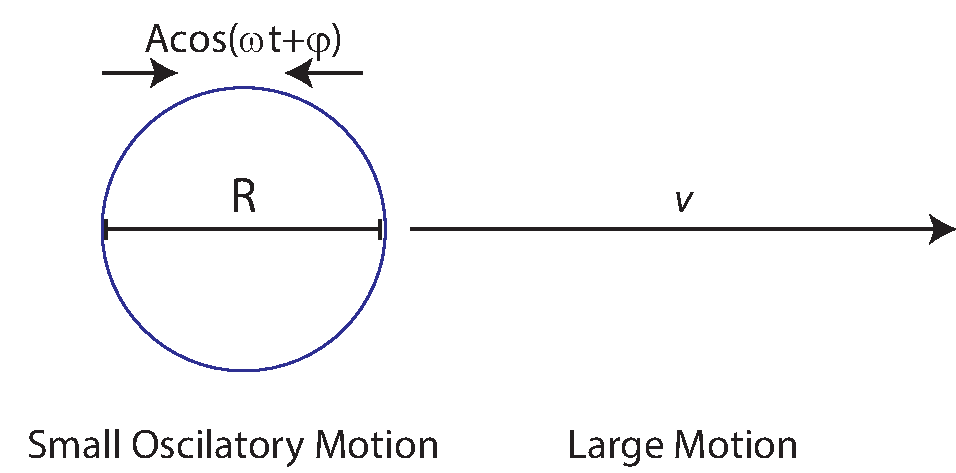
\includegraphics[width=0.49\columnwidth]{SmallOnLarge/SmallOnLarge.pdf}} & 
\multicolumn{2}{c}{\includegraphics[width=0.49\columnwidth]{SmallOnLarge/path.eps}}\\
\multicolumn{2}{c}{(a) Synthetic setup} & 
\multicolumn{2}{c}{(b) Plot of Motion} \\
\includegraphics[width=0.24\columnwidth]{SmallOnLarge/eulerPath1.eps} & 
\includegraphics[width=0.24\columnwidth]{SmallOnLarge/eulerPath2.eps} &
\includegraphics[width=0.24\columnwidth]{SmallOnLarge/eulerPathLoG1.eps} &
\includegraphics[width=0.24\columnwidth]{SmallOnLarge/eulerPathLoG2.eps}\\
\multicolumn{2}{c}{(c) Unwrapped Phase Signal} & 
\multicolumn{2}{c}{(d) LoG Filter applied to phase signal}\\
\end{tabular}
\caption{An example of Eulerian processing with large motions. A disk moves with constant velocity while undergoing a small oscillation (a-b). Despite the large motion, the phase signal at pixels that are near the disk in space and time contain the motion signal (c). We can recover the oscillatory motion by using a Laplacian of Gaussian filter (d). The filter width is determined automatically using }
\end{figure}



\end{document}